% !TEX program = xelatex
\documentclass[a4paper]{article}
\usepackage{amsthm}
\usepackage{amssymb}
\usepackage{bm}
\usepackage{mathtools}
\usepackage[x11names]{xcolor}
\usepackage{xparse}
\usepackage{fontspec}
\usepackage{unicode-math}
%\setromanfont{TeX Gyre ScholaX}
%\setromanfont{Gamaliel}
%\setromanfont{QTUSA-Uncial}
%\setromanfont{Elegante}
%\setromanfont{QTChanceryType}
%\setromanfont{MEBINAC_REGULAR.OTF}
\setromanfont{DovesType-Regular.otf}
\setsansfont{Andika}
\setmathfont{Asana Math}[Scale=1]

\usepackage{siunitx}
\usepackage{graphicx}
\usepackage[margin=1cm]{geometry}
\usepackage{tcolorbox} % or [most]{tcolorbox}
\tcbuselibrary{skins,xparse,poster}
\usetikzlibrary{fadings}

 \newcommand\fadingtext[3][]{%
   \begin{tikzfadingfrompicture}[name=fading letter]
     \node[text=transparent!0,inner xsep=0pt,outer xsep=0pt,#1] {#3};
   \end{tikzfadingfrompicture}%
   \begin{tikzpicture}[baseline=(textnode.base)]
     \node[inner sep=0pt,outer sep=0pt,#1](textnode){\phantom{#3}};
     \shade[path fading=fading letter,#2,fit fading=false]
     (textnode.south west) rectangle (textnode.north east);%
   \end{tikzpicture}%
 }

% \newcommand\fadingtextJ[3][]{%
%   \begin{tikzfadingfrompicture}[name=fading letterJ]
%     \node[text=transparent!0,inner xsep=0pt,outer xsep=0pt,#1] {#3};
%   \end{tikzfadingfrompicture}%
%   \begin{tikzpicture}[baseline=(textnode.base)]
%     \node[inner sep=0pt,outer sep=0pt,#1](textnode){\phantom{#3}};
%     \shade[path fading=fading letterJ,#2,fit fading=false]
%     (textnode.south west) rectangle (textnode.north east);%
%   \end{tikzpicture}%
% }
\newsavebox\mysavebox

\usepackage{lipsum}
\usepackage{varwidth}

\definecolor{JISpurple}{RGB}{89,72,122}
\definecolor{JISivory}{RGB}{241,234,221}
\definecolor{JIStaupe}{RGB}{183,156,154}

%\AddToHook{shipout/background}{%
%    \put (0in,-\paperheight){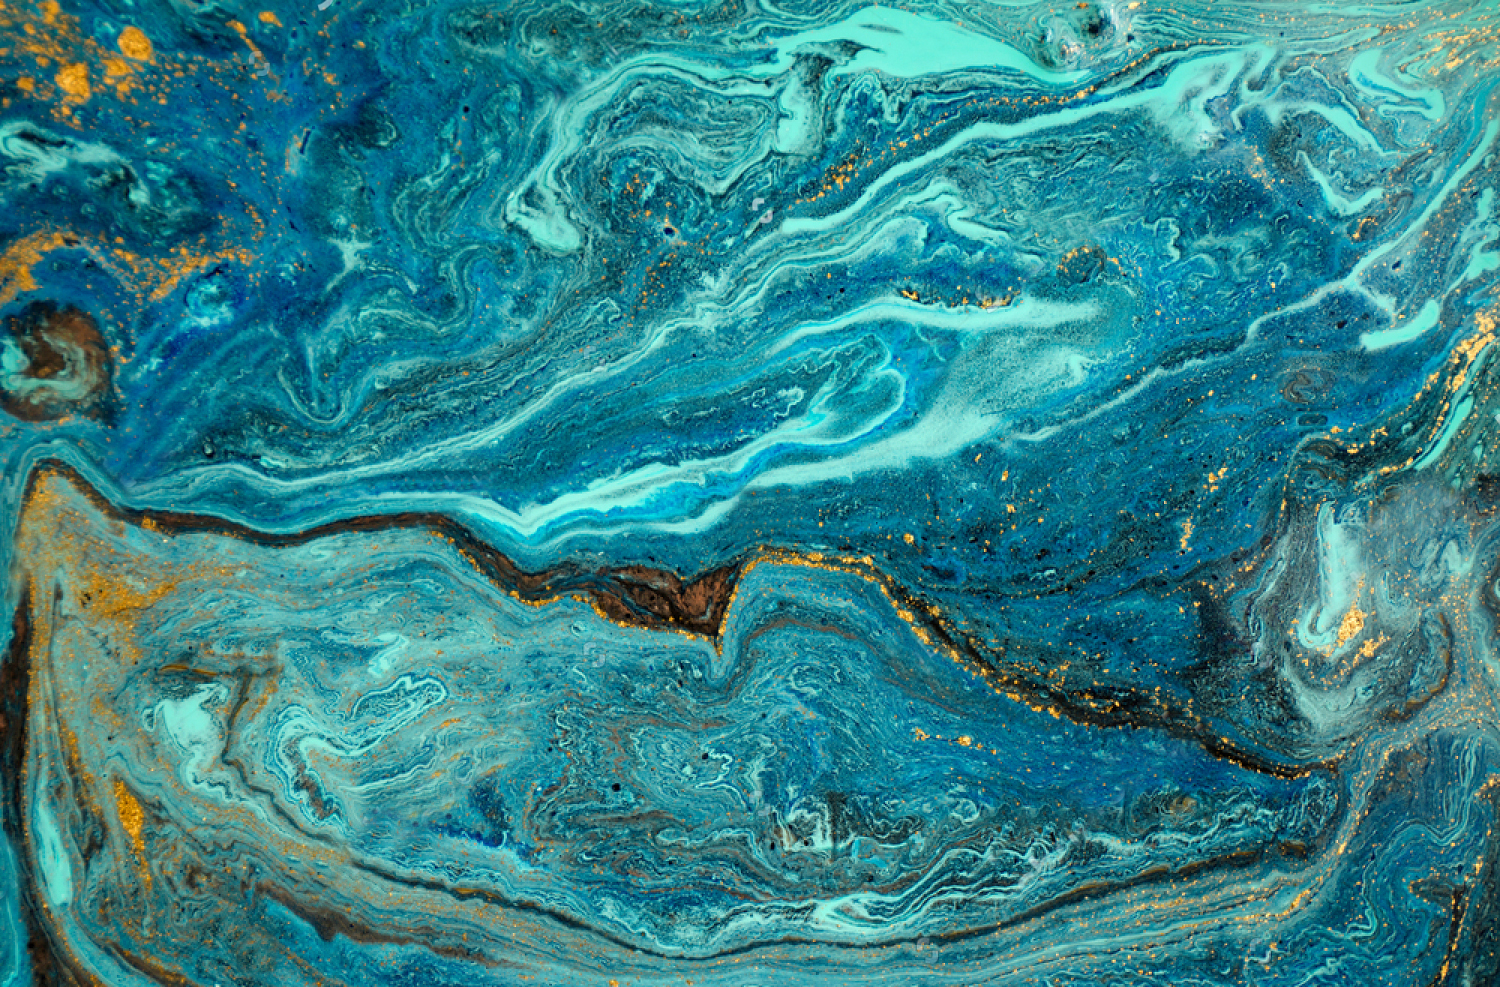
\includegraphics[width=\paperwidth,height=\paperheight]{images/bkg1.jpg}}%
%}

\newtcolorbox{My3Box}{%
  breakable,
  enhanced,
  colback=blue!0!white,
  colframe=JISpurple,
  %colframe=red!25!blue,
  title={
\includegraphics[width=0.9cm,height=0.9cm]{images/JIS Final Logo FA-02.png}\raisebox{3mm}{\large A Picture in the Title Bar}},
  %title={\smash{\raisebox{-7.5pt}{
\includegraphics[width=1cm,height=1cm]{images/JIS Final Logo FA-02.png}}}\hspace{0em}\huge Picture in Title},
}

\newtcolorbox{My4Box}[2][]{enhanced, interior hidden,
colframe=cyan!30, colback=cyan!30, coltitle=blue!70!black,
fonttitle=\bfseries\sffamily,
attach boxed title to top left,
boxed title style={empty, boxrule=0.5mm},
varwidth boxed title=0.5\linewidth,
underlay boxed title={
\path[draw=cyan!30, line width=0.5mm, rounded corners, fill=cyan!30]
([xshift=.25mm]frame.west) |- ([xshift=-2.5mm]title.north east) to[out=0, in=180] ([xshift=7.5mm, yshift=-.25mm]title.south east);
},
title={#2},#1}

\newtcolorbox{My5Box}[2][]{empty,
coltitle=JISpurple,
fonttitle=\bfseries\sffamily,
attach boxed title to top left={yshift=-2.5mm},
boxed title style={empty, size=small, top=1mm, bottom=0pt},
varwidth boxed title=0.5\linewidth,
frame code={
  \path (title.east|-frame.north) coordinate (aux);
\path[draw=JISpurple, line width=0.5mm, rounded corners]
(frame.west) |- ([xshift=-2.5mm]title.north east) to[out=0, in=180] ([xshift=7.5mm]aux)-|(frame.east)|-(frame.south)-|cycle;
},
title={#2},#1}

\title{JIS-WeeklyMathsChallenge-test1}
\author{N. J. Haes}
\date{July 2022}

\begin{document}
\begin{tcolorbox}[colback=blue!20!white,colframe=blue!70!black,title=\textbf{\huge{Weekly Maths Challenge}}]
    Some text.
    \begin{tcolorbox}
        Box in box.
    \end{tcolorbox}
    \begin{tcolorbox}[enhanced,title=Year 8 and above,frame style={left color = red!75!black,right color=blue!75!black}]
        \begin{tikzpicture}
          \path[fill tile image=pink_marble.png]
            (2.75,-0.75) -- (3,0) -- (2.75,0.75)
          \foreach \w in {45,90,...,315}
            { -- (\w:1.5cm) } -- cycle;
        \end{tikzpicture}
        \hfill
        Box upper
        \tcblower
        Box lower
        \begin{tikzpicture}
          \path[draw,fill plain image=goldshade.png]
            (2.75,-0.75) -- (3,0) -- (2.75,0.75)
          \foreach \w in {45,90,...,315}
            { -- (\w:1.5cm) } -- cycle;
        \end{tikzpicture}
    \end{tcolorbox}
\end{tcolorbox}

\begin{tcolorbox}[bicolor,sidebyside,righthand width=3cm,
sharp corners,boxrule=.4pt,colback=green!5,colbacklower=green!50!black!50]
  \lipsum[2]
  \tcblower
  \includegraphics[width=\linewidth]{goldshade}%
\end{tcolorbox}

Test.\\
%\noindent\fadingtext{top color=JISpurple,bottom color=white, middle color=JISpurple!75}{\parbox[b]{\linewidth}{\strut\lipsum[1]}}\\
% \noindent\fadingtext{bottom color=blue,top color=green}{\parbox[b]{\linewidth}{\strut\Huge{ Hello}}}\\
% \noindent\fadingtext{top color=JISpurple,bottom color=white, middle color=JISpurple!25}{\parbox[b]{\linewidth}{\strut\lipsum[1]}}\\

\DeclareTotalTColorBox{\mysidebox}{ O{} +m +m }{
bicolor,colback=white,colbacklower=yellow!10,
fonttitle=\bfseries,center title,
sidebyside,
code={\sbox{\mysavebox}{#2}},
lefthand width=\wd\mysavebox,
drop lifted shadow,
#1
}{
\usebox{\mysavebox}\tcblower#3}
\mysidebox[title=The Triangle]{%
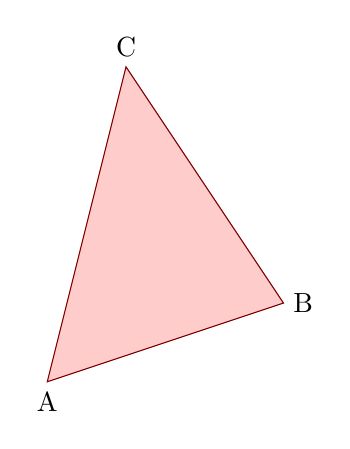
\begin{tikzpicture}
\path[fill=red!20,draw=red!50!black]
(0,0) node[below]{A} -- (3,1) node[right]{B}
-- (1,4) node[above]{C} -- cycle;
\end{tikzpicture}%
}{%
\lipsum[1]
}

\begin{tcolorbox}[enhanced,sharp corners=uphill,
    colback=blue!50!white,colframe=blue!25!black,coltext=yellow,
    fontupper=\Large\bfseries,arc=6mm,boxrule=2mm,boxsep=5mm,
    borderline={0.3mm}{0.3mm}{white}]
  Funny settings.
\end{tcolorbox}


\begin{tcolorbox}[enhanced,frame style image=blueshade.png,
  opacityback=0.75,opacitybacktitle=0.25,
  colback=blue!5!white,colframe=blue!75!black,
  title=My title]
  This box is filled with an external image.\par
  Title and interior are made partly transparent to show the image.
\end{tcolorbox}


\begin{tcolorbox}[enhanced,attach boxed title to top center={yshift=-3mm,yshifttext=-1mm},
  colback=blue!5!white,colframe=blue!75!black,colbacktitle=red!80!black,
  title=My title,fonttitle=\bfseries,
  boxed title style={size=small,colframe=red!50!black}]
  This box uses a \textit{boxed title}. The box of the title can
  be formatted independently from the main box.
\end{tcolorbox}

\begin{tcolorbox}[enhanced,attach boxed title to top left={yshift=-3mm,yshifttext=-1mm,xshift=3mm},
  colback=blue!5!white,colframe=blue!75!black,colbacktitle=red!80!black,
  title=Year 7 and below,fonttitle=\bfseries\sffamily\large,
  boxed title style={colframe=blue!50!black} ]
  This box uses a \textit{boxed title}. The box of the title can
  be formatted independently from the main box.
    \begin{align*}
    \rm\int_{a(t)}^{b(t)}f(x,t)dx, & \qquad\minus\infty< a(t),\quad b(t)<\infty\\
    \frac{d}{dt}\left(\int_{a(t)}^{b(t)}\!f(x,t)dx\right) &= f(t,b(t))\cdot\frac{d}{dt}b(t) \minus f(t,a(t))\cdot\frac{d}{dt}a(t) +\int_{a(t)}^{b(t)}\frac{\partial}{\partial t}f(x,t)dx\\
    \shortintertext{If \(a(t)\) and \(b(t)\) are constants rather than functions of \(t\)}
    \frac{d}{dt}\left(\int_{a}^{b}f(x,t)dx\right) &= \int_{a}^{b}\frac{\partial}{\partial t}f(x,t)dx
    \shortintertext{If \(a(t)=a\) and \(b(t)=t\)}
    \frac{d}{dt}\left(\int_{a}^{t}f(x,t)dx\right) &= \int_{a}^{t}\frac{\partial}{\partial t}f(x,t)dx + f(t,t)\\
  \end{align*}
\end{tcolorbox}
%
\begin{tcolorbox}[enhanced,watermark graphics=images/JIS-FinalLogoFA-07.png,
  watermark opacity=0.3,watermark zoom=1.1,
  colback=green!5!white,colframe=green!75!black,
  fonttitle=\bfseries, title=Box with a watermark picture]
  Here, you see my nice box with a picture as a watermark.
  This picture is automatically resized to fit the dimensions
  of my box. Instead of a picture, some text could be used or
  arbitrary graphical code. See the documentation for more options.
\end{tcolorbox}

%----------------------------------------------------------
\clearpage

\section{Boxes in boxes}
\begin{tcolorbox}[colback=yellow!10!white,colframe=yellow!50!black,
  every box/.style={fonttitle=\bfseries},title=Box]
  \begin{tcolorbox}[enhanced,colback=red!10!white,colframe=red!50!black,
    colbacktitle=red!85!black,
    title=Box inside box,drop fuzzy shadow]
    \begin{tcolorbox}[beamer,colframe=blue!50!black,title=Box inside box inside box]
      And now for something completely different: Boxes!\par\medskip
      \newtcbox{\mybox}[1][]{nobeforeafter,tcbox raise base,colframe=green!50!black,colback=green!10!white,
        sharp corners,top=1pt,bottom=1pt,before upper=\strut,#1}
      \mybox[rounded corners=west]{This} \mybox{is} \mybox{another} \mybox[rounded corners=east]{box.}
    \end{tcolorbox}
  \end{tcolorbox}
\end{tcolorbox}

\begin{tcbposter}[
  poster = {spacing=2mm,columns=3,rows=2},
  coverage = {%height=5cm    % setting this means contents overflow boxes
  interior style={top color=yellow,bottom color=yellow!50!red},
  },
  boxes = {sharp corners=downhill,arc=3mm,boxrule=1mm,
  colback=white,colframe=cyan,
  title style={left color=black,right color=cyan},
  fonttitle=\bfseries}
  ]
  \posterbox[adjusted title=First]{column=1,row=1,span=2}{First posterbox\\
    \lipsum[1]
  }
  \posterbox[adjusted title=Second]{column=1,row=2,span=2}{Maths in posterbox:\\
    \begin{align*}
      \rm\int_{a(t)}^{b(t)}f(x,t)dx, & \qquad-\infty< a(t),\quad b(t)<\infty\\
      \frac{d}{dt}\left(\int_{a(t)}^{b(t)}\!f(x,t)dx\right) &= f(t,b(t))\cdot\frac{d}{dt}b(t) - f(t,a(t))\cdot\frac{d}{dt}a(t) +\int_{a(t)}^{b(t)}\frac{\partial}{\partial t}f(x,t)dx\\
      \shortintertext{If \(a(t)\) and \(b(t)\) are constants rather than functions of \(t\)}
      \frac{d}{dt}\left(\int_{a}^{b}f(x,t)dx\right) &= \int_{a}^{b}\frac{\partial}{\partial t}f(x,t)dx
      \shortintertext{If \(a(t)=a\) and \(b(t)=t\)}
      \frac{d}{dt}\left(\int_{a}^{t}f(x,t)dx\right) &= \int_{a}^{t}\frac{\partial}{\partial   t}f(x,t)dx + f(t,t)\\
    \end{align*}
  }
  \posterbox[adjusted title=Third]{column=3,row=1,rowspan=2}{Third box\\ \lipsum[2]}
\end{tcbposter}

\newtcolorbox{My2box}[2][]{enhanced,skin=enhancedlast jigsaw,
attach boxed title to top left={xshift=-4mm,yshift=-0.5mm},
fonttitle=\bfseries\sffamily,varwidth boxed title=0.7\linewidth,
colbacktitle=blue!45!white,colframe=red!50!black,
interior style={top color=blue!10!white,bottom color=red!10!white},
boxed title style={empty,arc=0pt,outer arc=0pt,boxrule=0pt},
underlay boxed title={
\fill[blue!45!white] (title.north west) -- (title.north east)
-- +(\tcboxedtitleheight-1mm,-\tcboxedtitleheight+1mm)
-- ([xshift=4mm,yshift=0.5mm]frame.north east) -- +(0mm,-1mm)
-- (title.south west) -- cycle;
\fill[blue!45!white!50!black] ([yshift=-0.5mm]frame.north west)
-- +(-0.4,0) -- +(0,-0.3) -- cycle;
\fill[blue!45!white!50!black] ([yshift=-0.5mm]frame.north east)
-- +(0,-0.3) -- +(0.4,0) -- cycle; },
title={#2},#1}

\begin{My2box}{The A title}
  \lipsum[2]
\end{My2box}

\begin{My3Box}
    \Huge{The question.}
\end{My3Box}

\begin{My4Box}{Whose title?}
  \lipsum[2]
\end{My4Box}

\begin{My4Box}{A longer title}
  \lipsum[2]
\end{My4Box}

\begin{My5Box}{My title}
  \lipsum[2]
\end{My5Box}

\begin{My5Box}{Temporary Heading}
% \begin{My5Box}{\noindent\fadingtext{bottom color=JISpurple,top color=white, middle color=JISpurple!25}{\parbox[b]{0.4\linewidth}{\strut\huge Question}}}
  \lipsum[2]
\end{My5Box}

\newtcolorbox{My6Box}[2][]{skin=enhancedlast jigsaw,interior hidden,
boxsep=0pt,top=0pt,colframe=red,coltitle=red!50!black,
fonttitle=\bfseries\sffamily,
attach boxed title to bottom center,
boxed title style={empty,boxrule=0.5mm},
varwidth boxed title=0.5\linewidth,
underlay boxed title={
\draw[white,line width=0.6mm]
([xshift=0.3mm-\tcboxedtitleheight*2,yshift=0.3mm]title.north west)
--([xshift=-0.3mm+\tcboxedtitleheight*2,yshift=0.3mm]title.north east);
\path[draw=red,top color=white,bottom color=red!50!white,line width=0.5mm]
([xshift=0.25mm-\tcboxedtitleheight*2,yshift=0.25mm]title.north west)
cos +(\tcboxedtitleheight,-\tcboxedtitleheight/2)
sin +(\tcboxedtitleheight,-\tcboxedtitleheight/2)
-- ([xshift=0.25mm,yshift=0.25mm]title.south west)
-- ([yshift=0.25mm]title.south east)
cos +(\tcboxedtitleheight,\tcboxedtitleheight/2)
sin +(\tcboxedtitleheight,\tcboxedtitleheight/2); },
title={#2},#1}

\begin{My6Box}{My Walrus}
  \lipsum[2]
\end{My6Box}

\clearpage
\vspace{15mm}\\
% Like the above but moving the titlebox to the top.
\newtcolorbox{My7Box}[2][]{skin=enhanced jigsaw,interior hidden,
boxsep=0pt,top=0pt,colframe=JISpurple,coltitle=JISpurple!50!black,
fonttitle=\bfseries\sffamily,
attach boxed title to top left={yshifttext=-3mm,yshift=-0.5mm},
boxed title style={empty,boxrule=0.5mm},
varwidth boxed title=0.5\linewidth,
underlay boxed title={
\draw[white,line width=0.6mm]
([xshift=1.8cm-\tcboxedtitleheight*2,yshift=0.2mm]title.south west)
--([xshift=1.9cm+\tcboxedtitleheight*2,yshift=0.2mm]title.south east);
\path[draw=JISpurple,bottom color=white,top color=JISpurple,line width=0.5mm]
([xshift=1.8cm-\tcboxedtitleheight*2,yshift=0.25mm]title.south west)
cos +(\tcboxedtitleheight,\tcboxedtitleheight/2)
sin +(\tcboxedtitleheight,\tcboxedtitleheight/2)
-- ([xshift=2cm,yshift=0.25mm]title.north west)
-- ([xshift=1.95cm,yshift=0.25mm]title.north east)
cos +(\tcboxedtitleheight,-\tcboxedtitleheight/2)
sin +(\tcboxedtitleheight,-\tcboxedtitleheight/2); },
title={#2},#1}


% \begin{My7Box}{\hspace{4em}Kettle}
\begin{My7Box}{\fadingtext{top color=white, bottom color=JISpurple, middle color=JISpurple!25}{Haes}}
  \lipsum[1]
\end{My7Box}

\end{document}
